%%% LaTeX Template: Two column article
%%%
%%% Source: http://www.howtotex.com/
%%% Feel free to distribute this template, but please keep to referal to http://www.howtotex.com/ here.
%%% Date: February 2011

%%% Preamble
\documentclass[	DIV=calc,%
							paper=a4,%
							fontsize=12pt,%
							onecolumn]{scrartcl}	 					% KOMA-article class

\usepackage{lipsum}													% Package to create dummy text
\usepackage[english]{babel}										% English language/hyphenation
\usepackage[protrusion=true,expansion=true]{microtype}				% Better typography
\usepackage{amsmath,amsfonts,amsthm}					% Math packages
\usepackage[pdftex]{graphicx}									% Enable pdflatex
\usepackage[svgnames]{xcolor}									% Enabling colors by their 'svgnames'
\usepackage[hang, small,labelfont=bf,up,textfont=it,up]{caption}	% Custom captions under/above floats
\usepackage{epstopdf}												% Converts .eps to .pdf
\usepackage{subfig}													% Subfigures
\usepackage{booktabs}												% Nicer tables
\usepackage{fix-cm}													% Custom fontsizes
\usepackage[utf8]{inputenc}
\usepackage[top=2.5cm, bottom=2.5cm, left=2.5cm, right=2.5cm]{geometry}
\usepackage[ddmmyyyy]{datetime}
\addto\captionsenglish{%
	\renewcommand\tablename{Tabela}
	\renewcommand\figurename{Figura}
} 
 

 
%%% Custom sectioning (sectsty package)
\usepackage{sectsty}													% Custom sectioning (see below)
\allsectionsfont{%															% Change font of al section commands
	\usefont{OT1}{phv}{b}{n}%										% bch-b-n: CharterBT-Bold font
	}

\sectionfont{%																% Change font of \section command
	\usefont{OT1}{phv}{b}{n}%										% bch-b-n: CharterBT-Bold font
	}



%%% Headers and footers
\usepackage{fancyhdr}												% Needed to define custom headers/footers
	\pagestyle{fancy}														% Enabling the custom headers/footers
\usepackage{lastpage}	

% Header (empty)
\lhead{}
\chead{}
\rhead{}
% Footer (you may change this to your own needs)

%% ====================================
%% ====================================
%% mude o rodape  do projeto
%% ====================================
%% ====================================

\lfoot{\footnotesize \texttt{Cabeamento estruturado.} \textbullet ~Projeto Bloco "K" UTFPR/CP}


\cfoot{}
\rfoot{\footnotesize página \thepage\ de \pageref{LastPage}}	% "Page 1 of 2"
\renewcommand{\headrulewidth}{0.0pt}
\renewcommand{\footrulewidth}{0.4pt}



%%% Creating an initial of the very first character of the content
\usepackage{lettrine}
\newcommand{\initial}[1]{%
     \lettrine[lines=3,lhang=0.3,nindent=0em]{
     				\color{Black}
     				{\textsf{#1}}}{}}



%%% Title, author and date metadata
\usepackage{titling}															% For custom titles

\newcommand{\HorRule}{\color{DarkGoldenrod}%			% Creating a horizontal rule
									  	\rule{\linewidth}{1pt}%
										}

\pretitle{\vspace{-30pt} \begin{flushleft} 
				\fontsize{50}{50} \usefont{OT1}{phv}{b}{n} \color{NavyBlue} \selectfont 
				}

%% ====================================
%% ====================================
%% mude o titulo  do projeto
%% ====================================
%% ====================================

\title{Projeto Reestruturação Bloco "K" UTFPR/CP}					% Title of your article goes here

%% ====================================



\posttitle{\par\end{flushleft}\vskip 0.5em}

\preauthor{\begin{flushleft}
					\large \lineskip 0.5em \usefont{OT1}{phv}{b}{sl} \color{NavyBlue}}
\author{Pedro Holtz, Marcelo Machado, Filipe Bonacin, Ademir, Wellington, Jozua Henrique }  	% Author name goes here


\postauthor{\footnotesize \usefont{OT1}{phv}{m}{sl} \color{Black} 
					\\Universidade Tecnológica Federal do Paraná - Câmpus Cornélio Procópio 								% Institution of author
					\par\end{flushleft}}

\date{}																				% No date




%%% Begin document
\begin{document}
\maketitle
\thispagestyle{fancy} 	
\thispagestyle{empty}		% Enabling the custom headers/footers for the first page 
% The first character should be within \initial{}




%% ====================================
%% ====================================
%% mude o resumo  do projeto
%% ====================================
%% ====================================
\initial{E}\textbf{Este projeto tem como foco a implantação de uma nova estrutura de cabeamento de redes, que irá contemplar a infraestrutura da rede de hosts do “Bloco K" da UTFPR (Universidade Tecnológica Federal do Paraná) de Cornélio Procópio. Este projeto mostra o planejamento para a implantação de funcionalidades de rede, visando a velocidade, disponibilidade, escalabilidade, integridade, segurança e gerencia das informações. Os estudos deste projeto viabiliza a utilização dos serviços fornecidos pelos Servidores pré existentes no Campus da UTFPR/CP: Arquivos, cópias para restauração futura (backups), controle de acesso à internet, Controle de Usuários (AD), entre outros serviços e dados que irá ser utilizados na rede. Neste, é apresentado o projeto lógico e físico com base nas plantas baixas já existentes.}

%% ====================================
\begin{figure}
	\centering
	\includegraphics{utfpr}
\end{figure}

\vspace{3cm}
\centerline{\textit{\textbf{\today}}}

\clearpage
    \renewcommand*\listfigurename{Lista de figuras}
\listoffigures

\renewcommand*\listtablename{Lista de tabelas}
\listoftables




\clearpage
\renewcommand{\contentsname}{Sumário}
\tableofcontents
\clearpage

%% ====================================
%% ====================================
%% Inicio do texto
%% ====================================
%% ====================================
\section{Introdução}
O projeto se propõe, através de uma rede de computadores: servidores, shitches, outros dispositivos de rede e cabeamento, prover conectividade e interoperabilidade entre os mesmos, permitindo o intercambio de informações entre estes equipamentos de uma forma segura e rápida. Inerente a isto, serão utilizados recursos tecnológicos de informática a fim de implantar um ambiente estável, definir infraestruturas, padrões que possam ter escalabilidade, grande vida útil através de excelente custo benefício. O desenvolvimento do projeto segue princípios básicos de segurança em sistemas computacionais de rede de computadores, tais como: 
\begin{itemize}
\item \textbf{Velocidade:} Garantir a utilização de recursos modernos de comunicação. 
\item \textbf{Confidencialidade:} Proteger a informação disponibilizada; 
\item  \textbf{Disponibilidade:} Prevenir interrupções na operação da rede através de um plano de contingencia;
\item \textbf{Integridade:} propriedade que garante que a informação manipulada mantenha todas as características originais estabelecidas pelo proprietário da informação.
\end{itemize}
\subsection{Contribuições}
Serão oferecidos os mais diversos serviços de redes de computadores tais como: 
\begin{itemize}
\item Cabeamento estruturado de redes de computadores;
\item Compartilhamento de aplicativos e dispositivos dentro das empresas; 
\item Acesso a internet;
\item Gerenciamento e administração dos serviços/servidores;
\item Controle de tráfego e segurança da informação; 
\item Monitoramento do espaço físico por câmeras IP;
\item Entre outros serviços descritos no decorrer do projeto.
\end{itemize}	
\subsection{Benefícios}
\begin{itemize}
\item Gerenciamento mais eficiente dos ativos de rede.
\item Rapidez e facilidade na identificação de problemas na camada física do modelo OSI.
\item Diminuição nos custos de mão de obra e montagem de infra-estrutura. 
\item Substituição rápida de ativos de rede quando preciso, devido a ordenação dos cabos. 
\item Documentação técnica para que qualquer profissional, não necessariamente o que atuou na estruturação inicial, possa fazer novas implantações ou alterações. 
\item Localização fácil de um cabo, devido à identificação em todo o sistema. Facilidade na manutenção de uma área/estação de trabalho.
\end{itemize}

\section{Estado atual}
Infraestrutura ativos e passivos 
\begin{itemize}
	\item 01 Rack Attic 36U (600X800MM) com refrigeração 4 cooler na parte superior
	\item 07 switches 3Com 3CR17561-91 SuperStack 4500 26-Port
	\item 01 switch HP V1910-24G, modelo JE006A
	\item 01 switch HP A3600 Series, modelo JG301B - Switch “destinado apenas aos pontos de rede das câmeras IP e aos dois Access Points. Esse switch é POE.”
	\item 10 patch panels Furukawa 3CAT 6
	\item 16 organizadores de cabo para rack, DN Conectividade.
	\item Cabos Horizontais Furukawa Cat5e
	\item Cabos Câmeras IP Furukawa Cat6
	\item Cabos para acces Point Furukawa Cat6
	\item UPS 
\end{itemize}
\subsection{Infraestrutura lógica rede do bloco "K" UTFPR/CP}
\begin{itemize}
	\item K001 - 12 pontos para máquinas de alunos e 1 para o professor, 1 ponto para câmera ip
	\item K002 - 7 pontos para máquinas dos professores, 1 ponto para câmera ip
	\item K003 - 7 pontos para máquinas dos professores, 1 ponto para câmera ip
	\item K004 - 7 pontos para máquinas dos professores, 1 ponto para câmera ip
	\item Sala Secretários - 2 pontos de rede, 1 ponto para câmera ip
	\item K005 - 13 pontos, para máquinas dos professores ,1 ponto para câmera ip
	\item K006 - 12 pontos antigos para 3 professores. Antiga sala de pesquisa., 1 ponto para câmera ip
	\item K007 - Servidor de impressão, 8 pontos de rede sendo 2 pontos de professores e 2 pontos de impressora, 1 ponto para câmera ip
	\item K008 - 25 pontos de rede e máquinas, 1 ponto para câmera ip
	\item K009 - 25 pontos de rede e máquinas, 1 ponto para câmera ip
	\item Corredor: 2 pontos para câmera e 2 pontos para wifi
\end{itemize}
\subsection{Motivos para reestruturação}
\begin{itemize}
	\item Projetar e implantar uma nova topologia de rede , com a finalidade de ser alcançados serviços de rede com mais segurança, disponibilidade e robustez.
	\item A estrutura Atual apresenta problemas com as Eletro calhas ( amassadas, estufadas, saturadas) que podem influenciar na qualidade os cabos deixando-os expostos a interferências
\end{itemize}
\subsection{Observações:}
\begin{itemize}
	\item O chicote de cabos que sai pela parte de cima do rack vai para as salas K001, K002, K003, K004 e sala dos secretários (lado direito e centro do bloco, olhando do ponto de vista da entrada do bloco), passando por canaletas no alto. 
	\item O chicote de cabos que sai debaixo do rack vai para as salas K005, K006, K007, K008 e K009, numa canaleta que passa pela parede dessas salas.
\end{itemize}
 	
\section{Usuários e Aplicativos}
De acordo com os dados obtidos junto à coordenação e levantamento do setor de tecnologia foi elaborado o projeto para que se atenda a futuras demanda para crescimento previsto da \textbf{Sala k006} do \textbf{Bloco "K"}, projeto planejado e posto em vigor com as normas, tanto para a quantidade de pontos de rede como a infraestrutura necessária para instalação.
\subsection{Usuários}
Os usuários que utilizam a rede no \textbf{bloco "K"} são:
\begin{itemize}
\item Alunos (64 Usuários).
\item Professores (9 Usuários).
\item Técnicos administrativos.
\end{itemize}
\textbf{Total de 76 Usuários que irão utilizar a rede do Bloco K da UTFPR/CP.}

\subsection{Aplicativos}
Os aplicativos devem estar sempre atualizados, aplicando-se as correções porventura publicadas pelos fabricantes. Assim, garantindo a segurança e o desempenho dos mesmos.
Os serviços que serão utilizados no \textbf{Bloco "K"} são esses: 
\begin{itemize}
	\item \textbf{Active Directory (AD):} Armazenamento informações sobre objetos em rede de computadores e disponibiliza essas informações a usuários e administradores desta rede. Professores e  técnicos administrativos que trabalham no \textbf{Bloco "K"} utilizam Active Directory para conexões nas máquinas e cada um tem acesso às suas respectivas pastas compartilhadas e às impressoras.
	\item \textbf{Software Digifort:} Uso DVR Câmeras de segurança.
	\item \textbf{Servidor de impressão:} Compartilhamento de Impressoras para impressões e digitalizações, utilizando o S.O. Windows Server para controle impressoras locais e terceirizadas.
	\item \textbf{SAMBA e CIFS:} Compartilhamento de diretórios em rede.
	\item \textbf{FlexNet License:} Aplicativo de licenças flutuantes
	\item \textbf{Outros serviços de rede:} DHCP, DNS, FTP, TFTP, SSH, HTTP, HTTPS, Proxy, RPC, RDP, VNC. TeamViewer ,VOIP, Skype,  WEB WhatsApp.
\end{itemize}

\section{Estrutura predial existente}

Explique aqui a planta física dos prédios
Pode ser anexada, em escala ou não.

Deve conter uma descrição geral, indicando a possível distância entre os pontos de rede e restrições de instalação.

\section{Planta Lógica - Elementos estruturados}

\subsection{Estado atual}
\begin{figure}
	\centering
	\caption{Planta - Estado Atual "Bloco K"}
	\includegraphics{planta_atual2}
\end{figure}

\subsection{Topologia}
Proposta futura, proposta após implantação.
Deve conter o diagrama da rede. Atente-se a redundância  e ligações truncadas.
Deve explicar todos termos e componentes utilizados nestas plantas. Por exemplo: entrance facility, work area, horizontal cabling, etc..

Todos os elementos das figuras devem ser explicados. 
Crie esboço da configuração dos racks e brackets. Explique cada um dos componentes. Você pode criar uma tabela contendo figuras dentro, ou criar uma tabela e incluí-la como imagem. Por exemplo, verifique a tabela \ref{tab1}.

\input{tab1}

\subsection{Encaminhamento}
Eletrodutos, calhas, e qualquer material em que os cabos serão alojados/alocados.

\subsection{Memorial descritivo}

\begin{itemize}
	\item \textbf{Conector Fêmea CAT6 GigaLan} 
\end{itemize}

\begin{figure}
	\centering
	\caption{Conector Fêmea CAT6 GigaLan}
	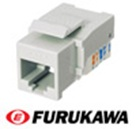
\includegraphics{keystone1}
\end{figure}

\textbf{Marca:} FURUKAWA 

\textbf{Quantidade:} 76 Peças.

Certificado RoHS alta qualidade.

\begin{itemize}
	\item \textbf{Módulo para espelhos modular 1U Branco 1 Porta} 
\end{itemize}

\begin{figure}
	\centering
	\caption{Módulo para espelhos modular 1U Branco 1 Porta}
	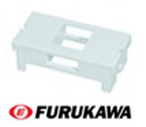
\includegraphics{espelho1}
\end{figure}

\textbf{Marca:} FURUKAWA

\textbf{Quantidade:} 76 Peças.

Este produto está em conformidade com a Diretiva Européia RoHs: uma medida restritiva ao uso de metais pesado na fabricação dos produtos e relacionadas à preservação do meio-ambiente.

\subsection{Identificação dos cabos}

\textbf{Uso Horizontal Permanente Furukawa}

\begin{figure}[!h]
	\centering
	\caption{Cabo Cat6}
	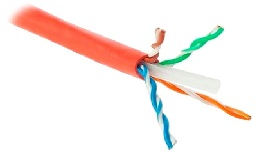
\includegraphics{cabo_cat6_1}
\end{figure}

\begin{itemize}
	\item Cabo de 4 pares trançados compostos de condutores sólidos de cobre nu, 23 AWG, isolados em polietileno especial. Capa externa em PVC não propagante à chama, nas opções CM, CMR e LSZH.
	\item Marcação sequencial métrica decrescente (305 - 0 m) com gravação de dia/mês/ano - hora de fabricação, proporcionando rastreamento do lote.
	\item Produto com capa CM tem padrão de fornecimento de acordo com a Diretiva RoHS.
\end{itemize}

\textbf{Uso Patch Cord Furukawa}

\begin{figure}[!h]
	\centering
	\caption{Patch Cord Furukawa}
	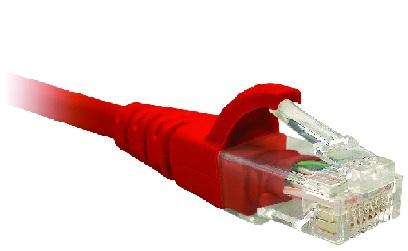
\includegraphics{patch_cord_cat6_1}
\end{figure}

\begin{itemize}
	\item Possui "boot" injetado, no mesmo dimensional do plug RJ-45 para evitar fadiga no cabo em movimentos de conexão e que evitam a desconexão acidental da estação de trabalho. 
	\item Produzido com Cabo Fast-Lan Extra-flexível U/UTP certificado pela Anatel.
	\item ROHS Compliant.
\end{itemize}

\textbf{Rotulação dos Cabos}

\begin{figure}[!h]
	\centering
	\caption{Rotulação dos Cabos}
	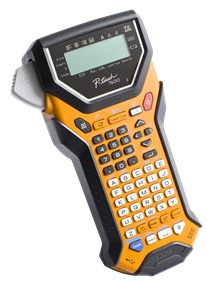
\includegraphics{rotulador_1}
\end{figure}

\begin{itemize}
	\item O rotulador PT7600 é robusto, portátil e utilizar as variadas e resistentes fitas TZ.
	\item Cria etiquetas com gráficos e códigos de barra de até 24mm de largura. Permite transferir para a memória do rotulador, etiquetas criadas através do software editor com figuras, gráficos e fotos.
	\item Logo após a instalação dos cabos e a certificação rotular os cabos nas extremidades para fácil identificação no Wallplates e nos Patch Panel
\end{itemize}

\section{Implantação}
Estabeleça um cronograma de implantação:
Remoção de equipamentos existentes (destino para descarte), instalação dos condutores, instalação dos cabos, 
identificação dos cabos, montagem dos racks, certificação, etc... Crie atividades e estabeleça o tempo de execução. Se for um projeto real, indique também quais os responsáveis pela execução do projeto e de cada uma das etapas.

Defina marcas (e padrões) e fornecedores se for o caso. Atenção a contratados e subcontratados para a realização das atividades. Estabeleça a responsabilidade de execução da atividade e também da validação dela.

Utilize algum software para gerear o cronograma. Excel,etc. O fundamental é dividir em etapas, descrever e estimar o tempo de cada uma delas.

Segue uma relação de ferramentas:
http://asana.com/, 
https://trello.com/, 
http://www.ganttproject.biz/, 
http://www.orangescrum.org/. 

\section{Plano de certificação}
A baixo foi relacionado as etapas seguidas para a certificação:
\begin{itemize}
\item \textbf{Paradiafonia (NEXT)};
\item \textbf{Verifica a quantidade de conexões no link};
\item \textbf{Impedância do cabo:} Expressa a contribuição das resistências, indutâncias, capacitâncias e condutâncias distribuídas ao longo do condutor, e medida em campo por meio de cable scanners. A qualidade de construção do cabo, é principal determinante no valor da impedância do mesmo.
\item \textbf{Atenuação do cabo:} Perda de potência do sinal transmitido – quanto maior a frequência do sinal pior é o caso (efeito skin ).
\item \textbf{ACR (atenuação x NEXT):} Importante parâmetro a ser medido que expressa relação entre a Atenuação e o NEXT .
\item \textbf{Return Loss (perda de retorno):} Reflexões causadas por anomalias na impedância característica ao longo de um segmento de cabo.
\end{itemize}
Após o termínio da passagem dos novos cabos e climpagem de seus conectores. A certificação de rede será realizada em toda rede. Desde sua origem (Patch Panel) até o destino (novos pontos de rede) contemplados no projeto no Bloco "K" da UTFPR/CP. 
A certificação partirá do Patch Panel localizado na \textbf{Sala k007} do \textbf{bloco "k"} até cada novo ponto de rede criado nas salas contempladas no projeto. 
Segue a tabelas de horários e dias da semana para a certificação:

\begin{table}[!h]
\centering
\caption{Primeiro dia}
\label{my-label}
\begin{tabular}{|l|l|l|}
\hline
\textbf{Sala}    &\textbf{Inicio}                     &\textbf{Fim}              \\ \hline
k001                     & 8Hs,                       & 10Hs.                    \\ \hline
k002                     & 10Hs.                      & 12hs.                    \\ \hline
k003                     & 14Hs                       & 16Hs.                    \\ \hline
k004                     & 16Hs.                      & 18Hs.                    \\ \hline
\end{tabular}
\end{table}
\begin{table}[!h]
\centering
\caption{Segundo dia}
\label{my-label}
\begin{tabular}{|l|l|l|}
\hline
\textbf{Sala}    &\textbf{Inicio}                     &\textbf{Fim}              \\ \hline						
k005                     & 8Hs,                       & 10Hs.                    \\ \hline
k006                     & 10Hs.                      & 12Hs.                    \\ \hline
k008                     & 14hs.                      & 16Hs.                    \\ \hline
k009                     & 16Hs.                      & 18Hs.                    \\ \hline
\end{tabular} 
\end{table}

Ao finalizar as certificações de rede será gerado o seguinte relatório:

\section{Plano de manutenção}

Por meio dos serviços de analise e diagnóstico de rede, é realizado um trabalho forense de cada dispositivo na rede por criticidade de sua operação que permite diagnosticar os gargalos e sugerir ações práticas de correção.
Será realizado trimestralmente a manutenção e execução de serviços de analise e diagnóstico de rede. Desta forma, é possível garantir elevado nível de serviço exigido pela rede para atender o tráfego de voz, imagem e outros dados.
Quando necessário adicionar um novo ponto de rede, deverá respeitar as normas utilizadas no projeto. Após a adição de um novo ponto de rede, se faz necessário realizar teses conforme a certificação utilizada no projeto. Assim, é possível garantir que tudo após o serviço a rede continua funcionando de forma esperada.
O propósito de um sistema de cabeamento estruturado é garantir uma base sólida para o bom desempenho das redes de comunicação de voz, imagem e outros dados devem permitir mudanças e alterações de layout nas demandas de mudança.
\subsection{Manutenção corretiva}
Os procedimentos acima contribuem para viabilizar a manutenção corretiva, que é aquela de atendimento imediato para consertar equipamentos danificados ou que sofreram avarias. Normalmente, o número de avarias cresce à medida que não são tomadas medidas antecipadas para o perfeito funcionamento dos equipamentos.
Este tipo de manutenção é considerado como um dos que mais onera a produção, porque, normalmente, tal manutenção implica na parada do equipamento e interrupção da produção. Por isso, a equipe de manutenção deve trabalhar com eficácia para evitar que os equipamentos sempre parem precisando de manutenção corretiva.
\subsection{Manutenção preventiva}
O treinamento da equipe de manutenção deve ser contínuo, pois tal procedimento é indispensável para garantir maior disponibilidade e confiabilidade dos equipamentos existentes na rede. Para um efetivo controle da manutenção preventiva é necessário monitorar o tráfego de rede e analisar o desempenho no que tange as transmissões por meio físico da rede. 
\subsection{Equipe de suporte}
A equipe de suporte de redes, terão que estar preparados para resolver possíveis problemas que possam ocorrer durante as atividades dos funcionários e alunos da UTFPR/CP. Caso ocorra uma ocorrência em um ponto de rede, o suporte técnico deve identificar o local onde ocorreu o problema, e o mais rápido possível a equipe de suporte se deslocar até o local afetado, analisar o problema e resolvê-lo.


\subsection{Plano de expansão}
Existe um plano de expansão? Quantos novos pontos poderão ser acrecidos na rede, antes de migração de equipamentos na camada 2? Se houver expansão, quais equipamentos deverão ser direcionados para as estremidades da rede? 


\section{Orçamento}
Crie uma relação de orçamentos baseado na seções anteriores.

\section{Referências bibliográficas}
Utilize o mendley, o jabref ou diretamente o bibtex para gerenciar suas referências biliográficas. As referências são criadas automaticamente de acordo com o uso no texto.

Exemplo: Redes de computadores, segundo \cite{t2013} é considerada..... Já \cite{kurose2010} apresenta uma versão...

Analisando os pressupostos de \cite{ref3} e \cite{ref4} concluimos que....


\renewcommand\refname{} %%Referências bibliográficas}  
\bibliographystyle{ieeetr}
\bibliography{referencias}  

%% ***********************************************************************
%% === remover daqui =====================================================
%% ***********************************************************************

\section{Elementos textuais - Alguns exemplos}

Esta seção apresenta exemplos de elementos textuais. \textbf{Remova-a da versão final do texto}.


\subsection{Colocar elementos em itens}

Texto antes da lista

\begin{itemize}
	\item First item in a list 
	\item Second item in a list 
	\item Third item in a list
\end{itemize}

\subsubsection{Uma sub seçao de terceiro nivel}

Exemplo de uma subseção

\subsection{Tabelas}

Utilize o site http://www.tablesgenerator.com/ para elaborar as tabelas de seu trabalho.
Para adicionar uma tabela utilize: a tag input, passando o arquivo da tabela como parametro

\input{tab2}

Dentro do arquivo você deve definir o label e pode utilizá-lo para referenciar. Exemplo:
Na tab \ref{tab2} temos a relação de ....


Você também pode modificar a tabela manualmente, incluindo, por exemplo h! dentro de sua definição. Veja no exemplo tab2.tex

\subsection{Figuras}

As figuras podem ser no formato PDF, JPG, PNG. Você pode referenciá-las da mesma maneira que tabelas. Exemplo: A figura \ref{fig1} apresenta.....

Não se preocupe o local em que a figura será renderizada em seu texto. Preocupe-se em criar referência para ela, ou seja, toda figura e tabela deve conter pelo menos uma referência no texto.

\begin{figure}
\centering
\includegraphics[width=\textwidth]{fig1}
\caption{Exemplo de figura com escala horizontal}
\label{fig1}
\end{figure}


\begin{figure}
	\centering
	\includegraphics[]{fig2}
	\caption{Exemplo de figura sem escala}
	\label{fig2}
\end{figure}

Você pode rotacionar figuras também. Para isso utilize o parâmetro angle=-90. Repare que a escala da figura foi modificada pelo parametro height. Você também pode utilizar scale

\begin{figure}
	\centering
	\includegraphics[height=\textwidth,angle=-90]{fig3}
	\caption{Exemplo de figura rotacionada}
	\label{fig3}
\end{figure}


%% ***********************************************************************
%% === ate aqui    =====  ================================================
%% ***********************************************************************
\end{document}